% \section{Introduction}
%
% \section{Methods}
%
% \subsection{Target selection}
%
% The dataset for this experiment was compiled of all modelling runs from all targets used in previous studies. All decoy sets restrained with contact predictions from either CCMPRED \cite{Seemayer2014-ml}, MEMBRAIN \cite{Yang2013-lv}, METAPSICOV \cite{Jones2015-wp} or PCONSC2 \cite{Skwark2014-mu} and the FADE energy function were considered. In total, this gave a set of 56 targets with a maximum of four contact predictions each. However, not all predictors were applicable to all targets, such as the \textalpha-helical transmembrane predictor MEMBRAIN \cite{Yang2013-lv} to globular targets. Thus, a final dataset of 113 decoy sets (1,000 decoys each) was created.
%
% \subsection{Decoy subselection}
%
% The precision score of long-range contact pairs ($\geq24$ residues sequence separation) was calculated for every decoy in every decoy set using ConKit (see Chapter XYZ). Subsequently, decoy sets were reduced for Molecular Replacement trials. Four different algorithms were used: \textit{NONE}, \textit{LINEAR}, \textit{SCALED}, and \textit{CUTOFF}. The \textit{NONE} algorithm accepted all 1,000 decoys and left the original set unchanged, which is identical to the current AMPLE approach. The \textit{LINEAR} algorithm sliced a decoy list removing the 500 decoys satisfying the least number of long-range contacts. For the \textit{SCALED} algorithm, each long-range contact precision score was divided by the set's average score, and only decoys with scores $\geq0.5$ kept. The \textit{CUTOFF} algorithm excluded all decoys with a long-range contact precision score of $<0.287$, a hard-coded threshold identified by \cite{De_Oliveira2017-yf} Thus, for every starting decoy set, we obtained four different decoy sets for Molecular Replacement trials using AMPLE.
%
% \subsection{Molecular Replacement}
%
% For the Molecular Replacement trials, a modified version of AMPLE was used. The modified version created ensemble search models for all 10 clusters. Trialling decoys from all 10 clusters was aimed to broaden the search space by including more conformations. Simultaneously, previous results suggested that polyalanine side-chain treatment by itself was nearly as good as all three side-chain treatments. Thus, to reduce the number of ensemble search models to trial, the most-reliable side-chain treatment was excluded. Similarly, the 2\AA subclustering radius appeared to be redundant in almost all cases, and thus this set of ensembles was also removed. Additionally, clustering was performed using a modified version of Spicker, which clusters decoys using TMscore values instead of RMSD values. Although at an increased runtime, this modification has shown to be beneficial to the clustering step (Jens MH Thomas; PhD Thesis). All modifications explained here were made publicly available in AMPLE v1.2.0 and CCP4 v7.0.32.
%
% To trial the different subselection algorithms, we decided to trial one contact prediction decoy set for 21 targets, which created a total of 63 AMPLE runs (three for each set). The target and resulting decoy sets were identical to the one published by @Simkovic2016. Besides the modifications outlined above, AMPLE was run with default settings.

\section{Results}

In this experiment, we assessed the value of subselecting sets of 1,000 decoys to AMPLE's cluster-and-truncate approach. Decoys were subselected using one of four algorithms, namely \textit{NONE}, \textit{LINEAR}, \textit{SCALED} or \textit{CUTOFF}. Each algorithm considered the long-range contact precision in a decoy and used it to exclude different numbers from the original set.

\subsection{Long-range contact precision and its relationship to decoy quality}

The underlying principle of this study is the positive linear relationship between long-range contact precision and the decoy quality. Here, we can validate previous findings of this relationship \cite{} given the precision of long-ralong-range contact prediction and the decoy quality.

Almost all targets across four contact prediction algorithm show positive linear relationships (Fig \ref{fig:ample_decoys_lrprectm}). This relationship applies to globular and transmembrane protein folds.

% \begin{figure}[H]
%     \centering
%     \begin{subfigure}[b]{\textwidth}
%         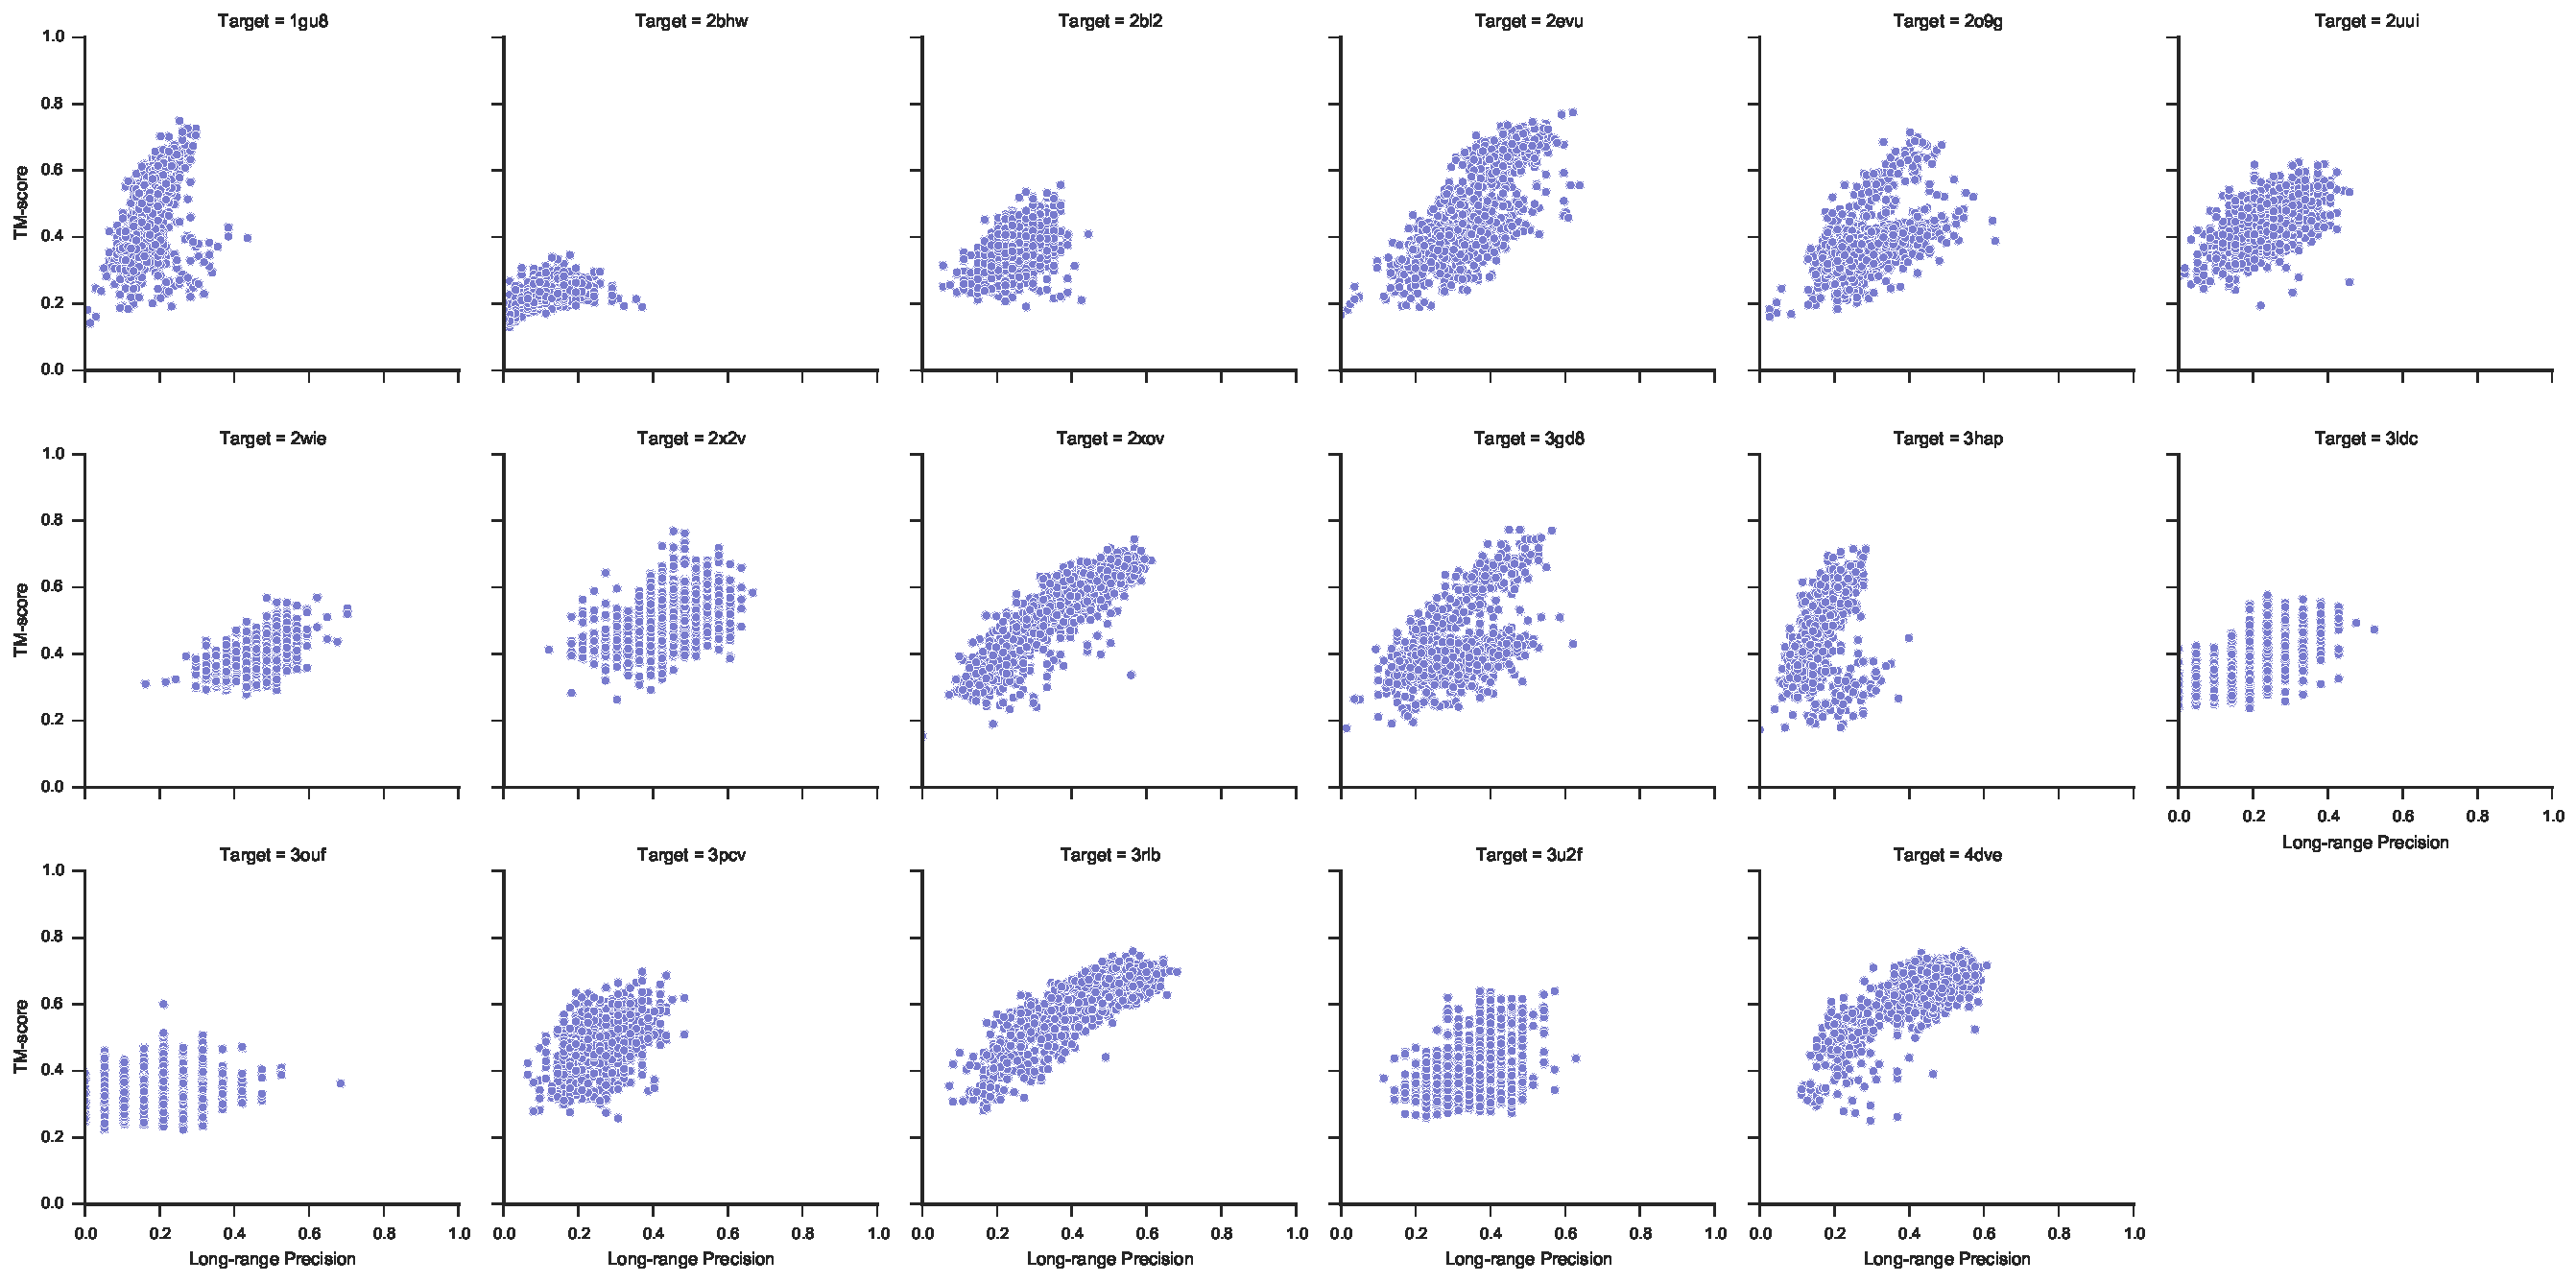
\includegraphics[width=\textwidth]{ample_decoys_ccmpred_lrprectm.pdf}
%         \caption{}
%         \label{fig:ample_decoys_ccmpred_lrprectm}
%     \end{subfigure}
%     \begin{subfigure}[b]{\textwidth}
%         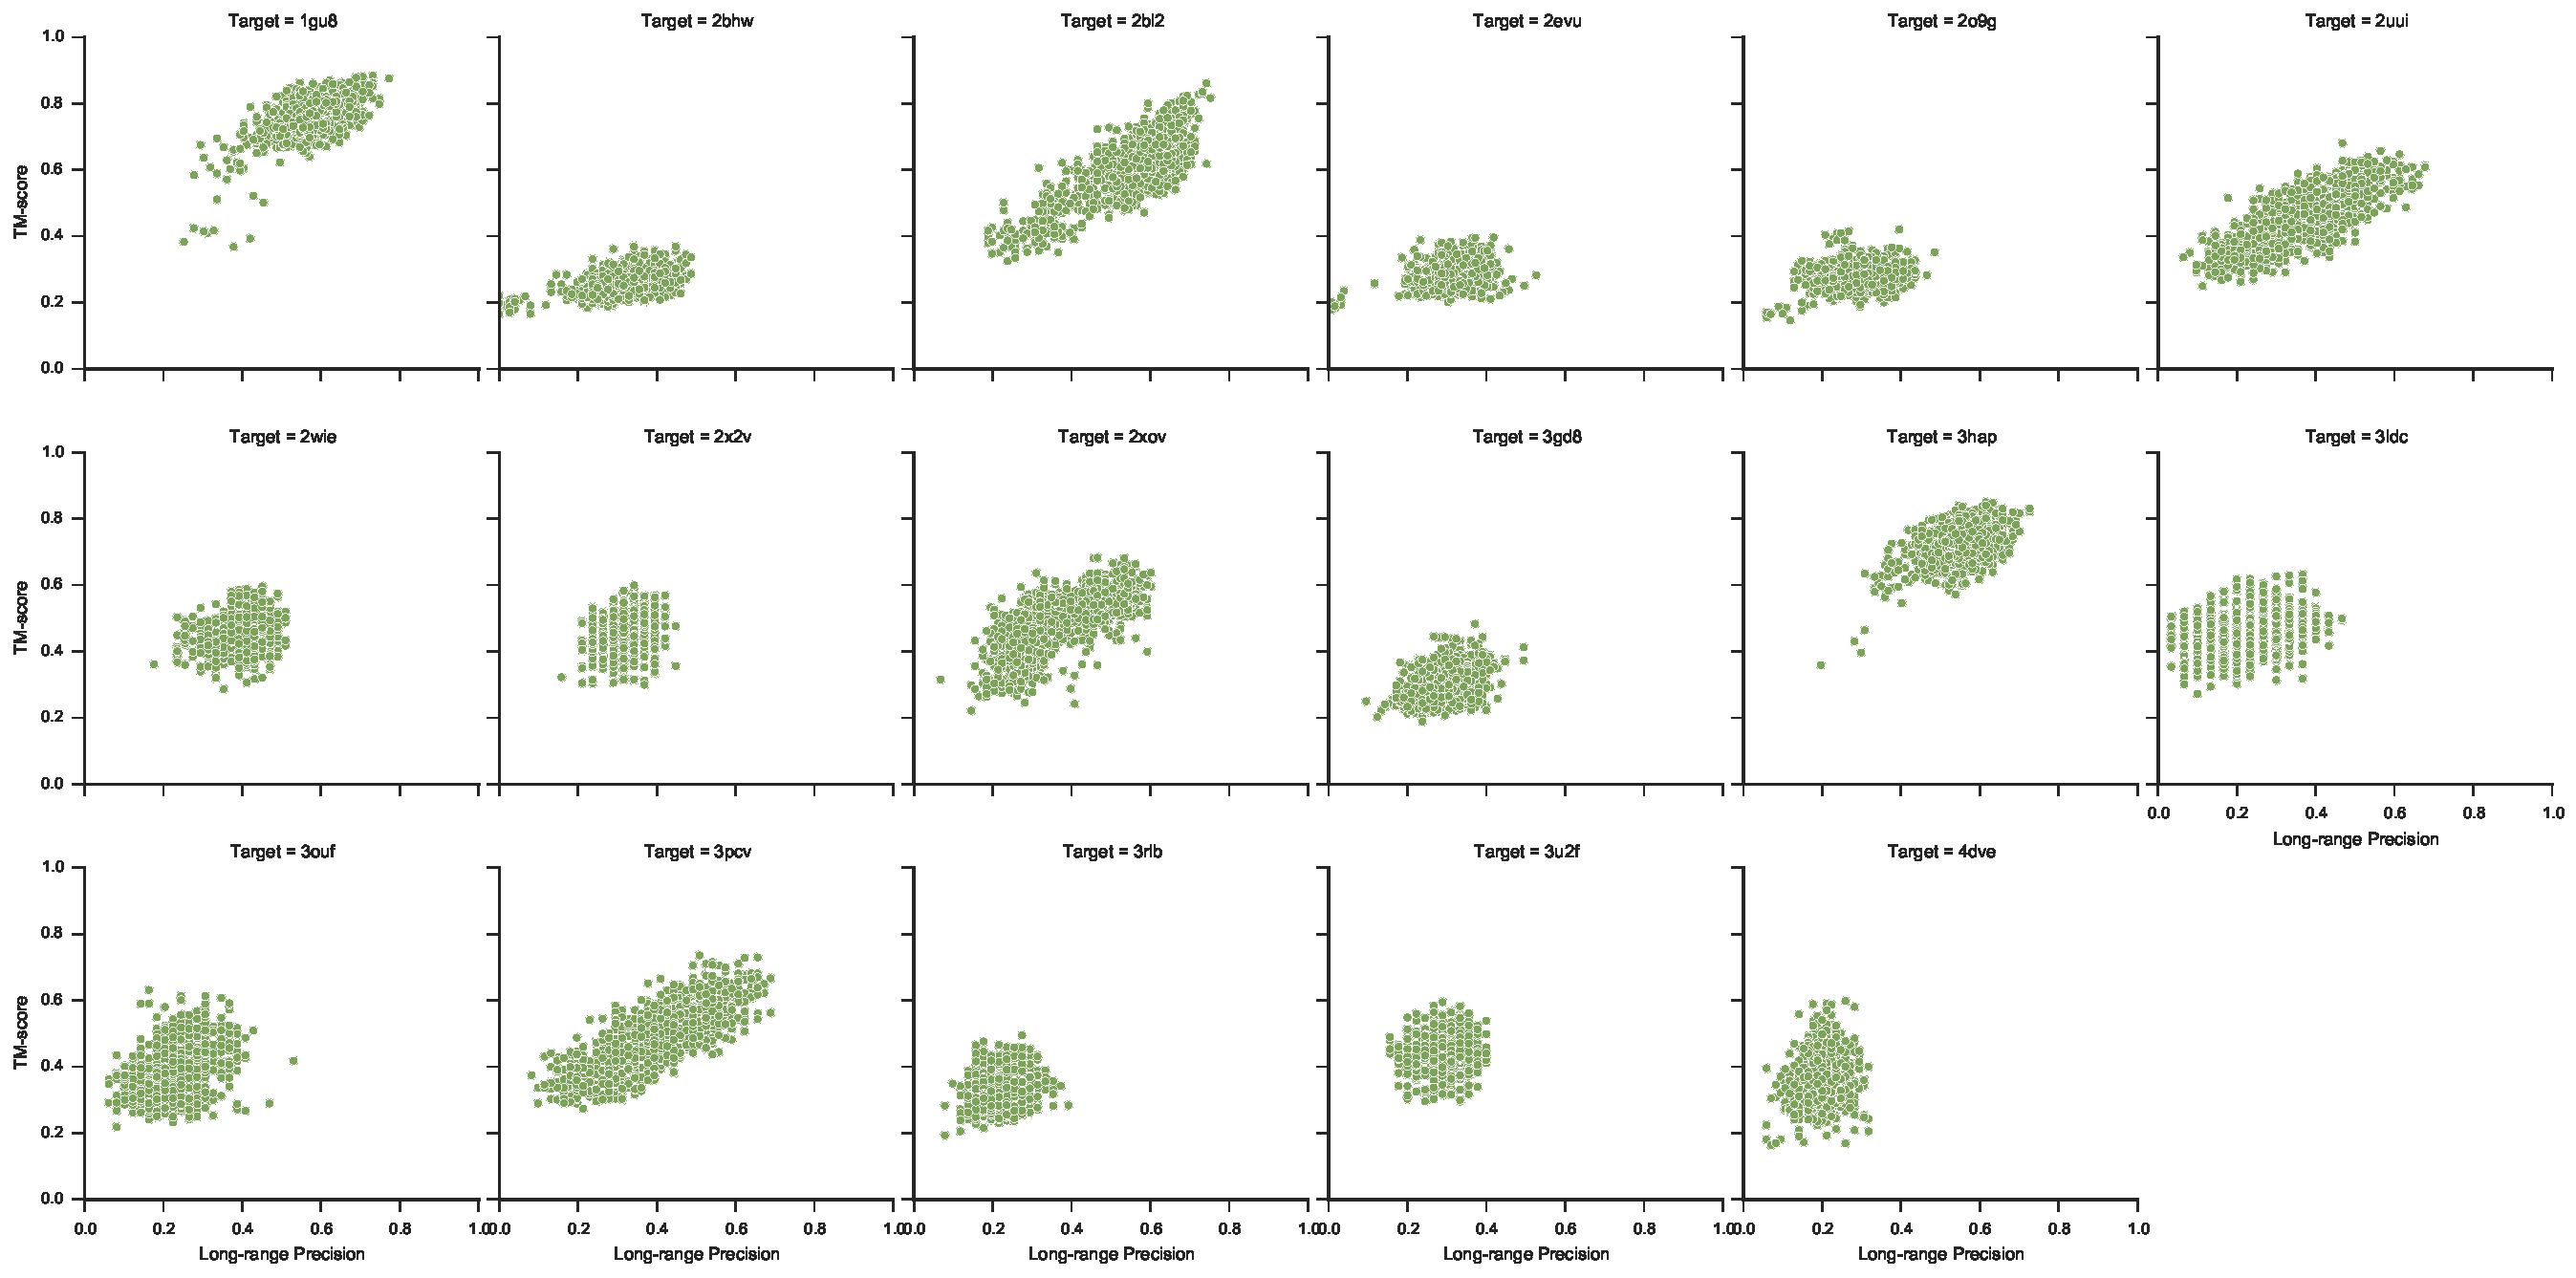
\includegraphics[width=\textwidth]{ample_decoys_membrain_lrprectm.pdf}
%         \caption{}
%         \label{fig:ample_decoys_membrain_lrprectm}
%     \end{subfigure}
% \end{figure}
% \begin{figure}[H]
%     \ContinuedFloat
%     \begin{subfigure}[b]{\textwidth}
%         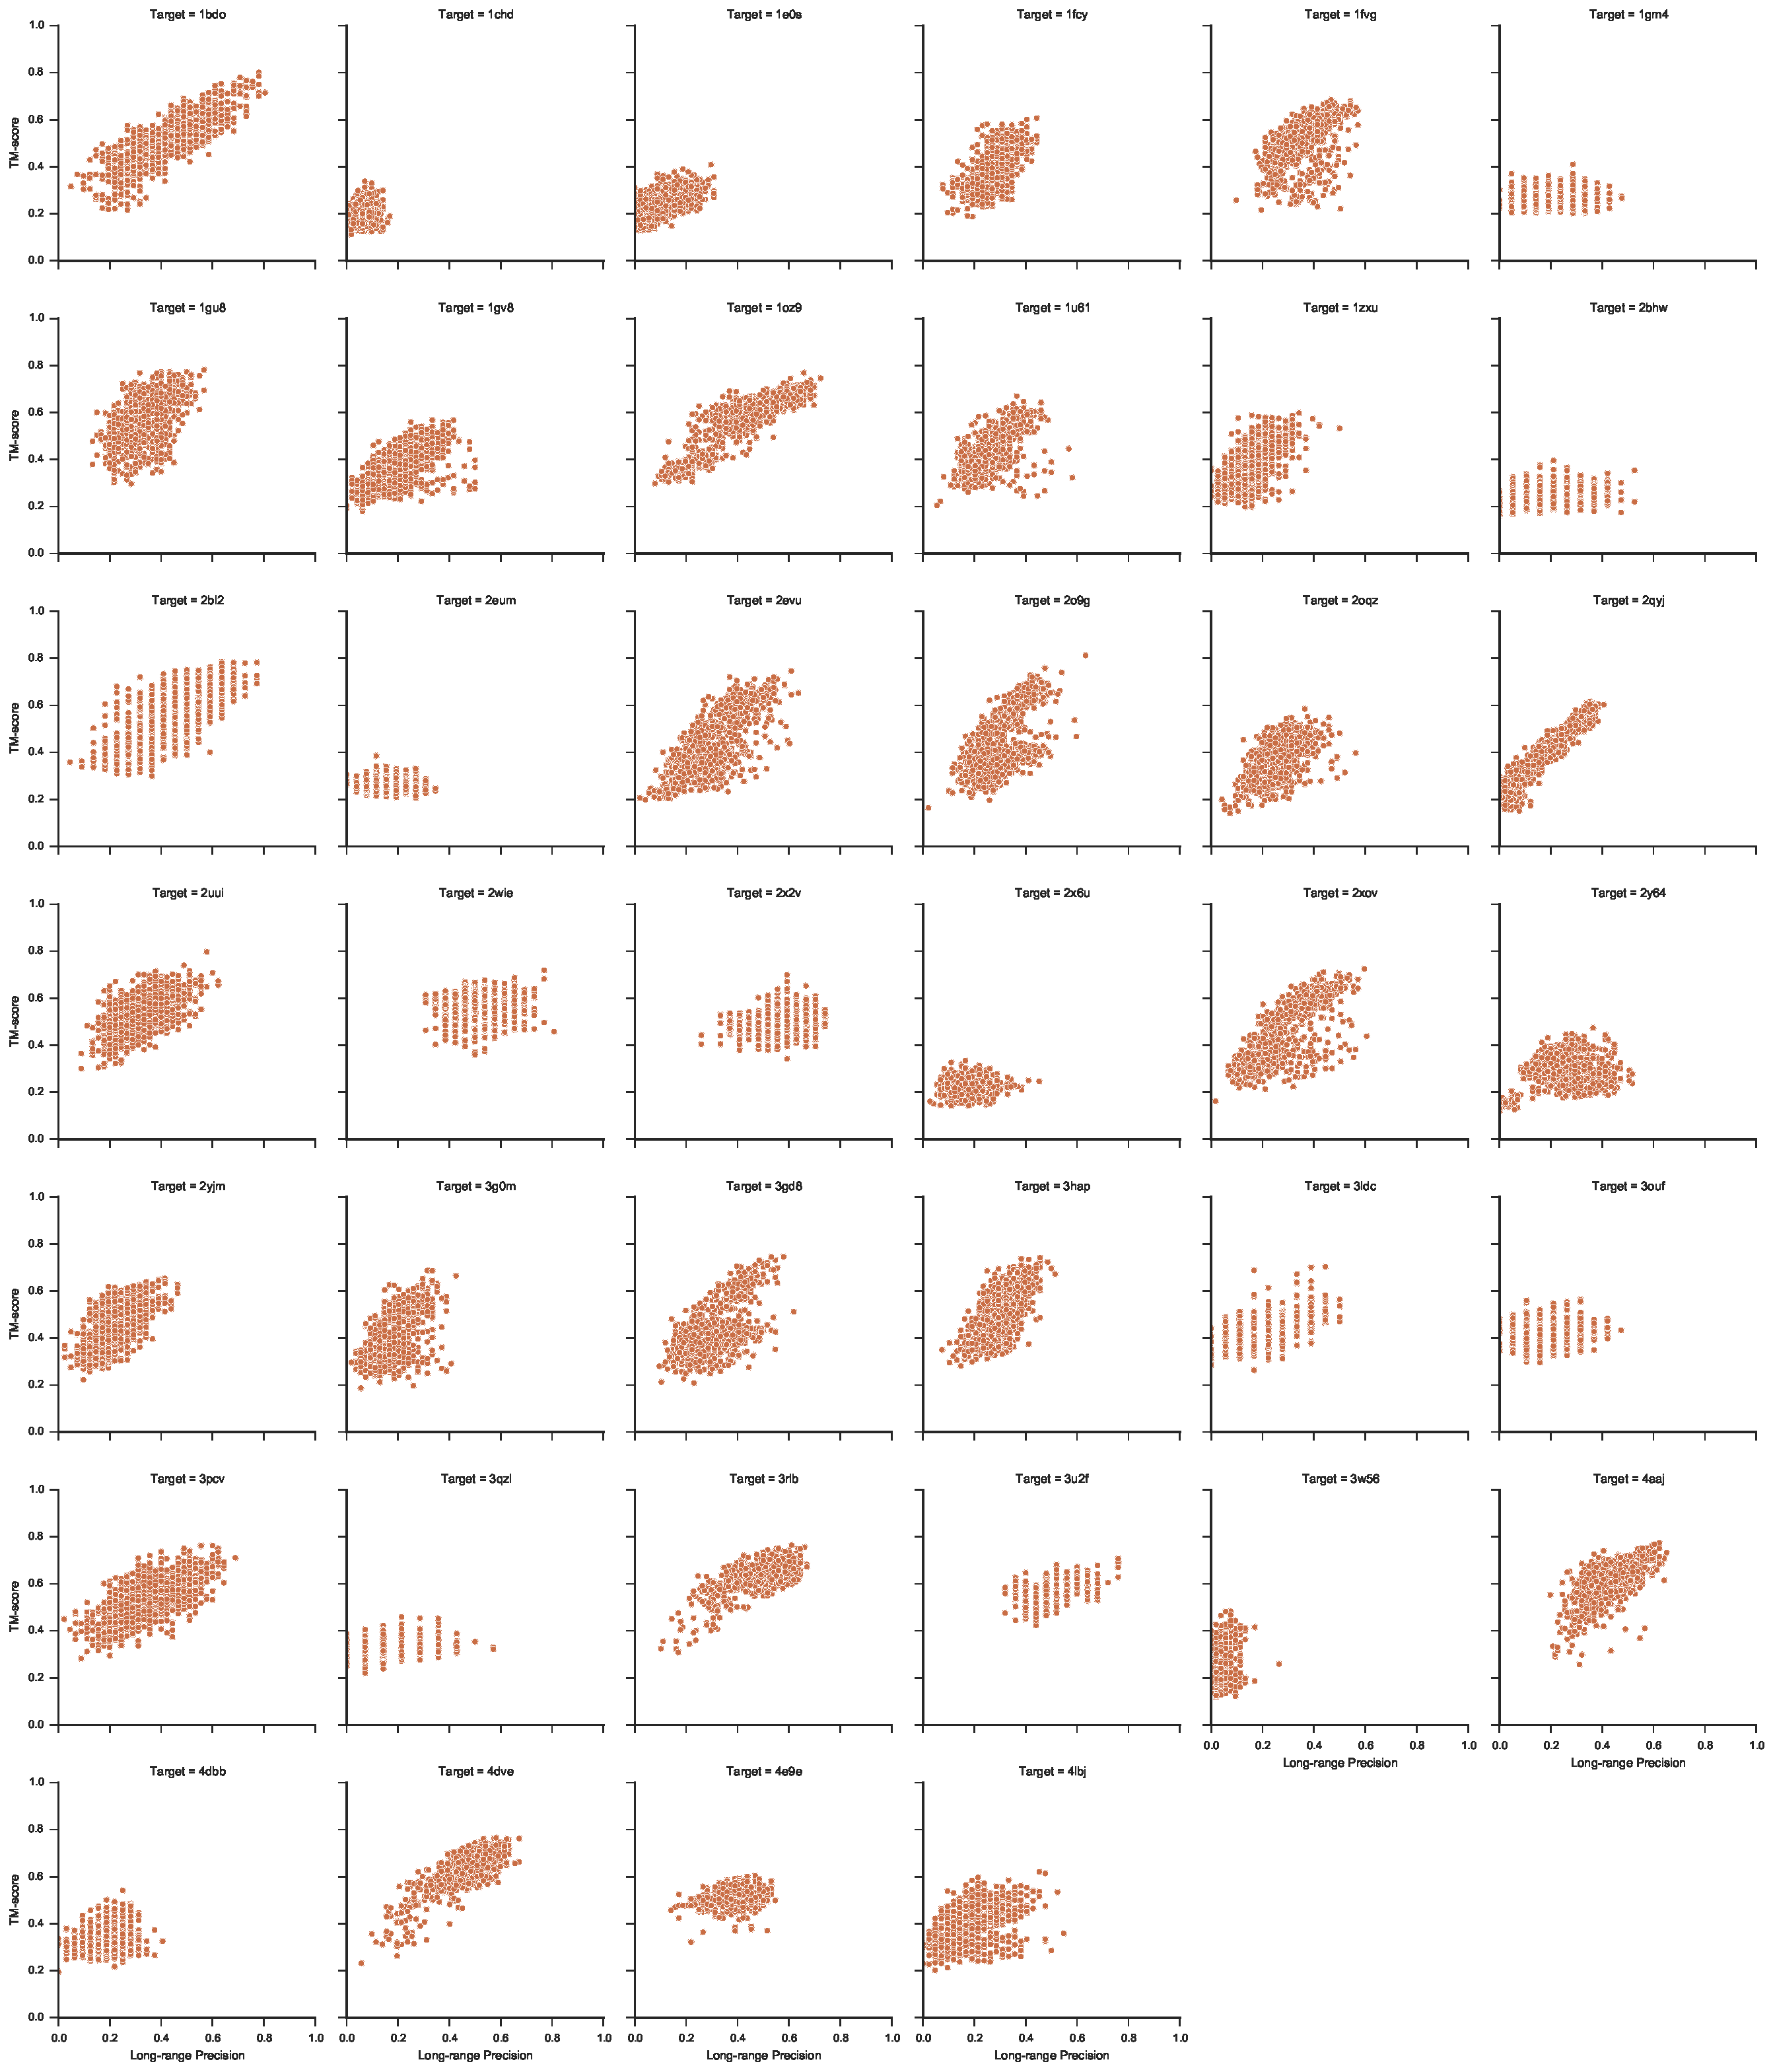
\includegraphics[width=\textwidth]{ample_decoys_metapsicovstage1_lrprectm.pdf}
%         \caption{}
%         \label{fig:ample_decoys_metapsicovstage1_lrprectm}
%     \end{subfigure}
% \end{figure}
% \begin{figure}[H]
%     \ContinuedFloat
%     \begin{subfigure}[b]{\textwidth}
%         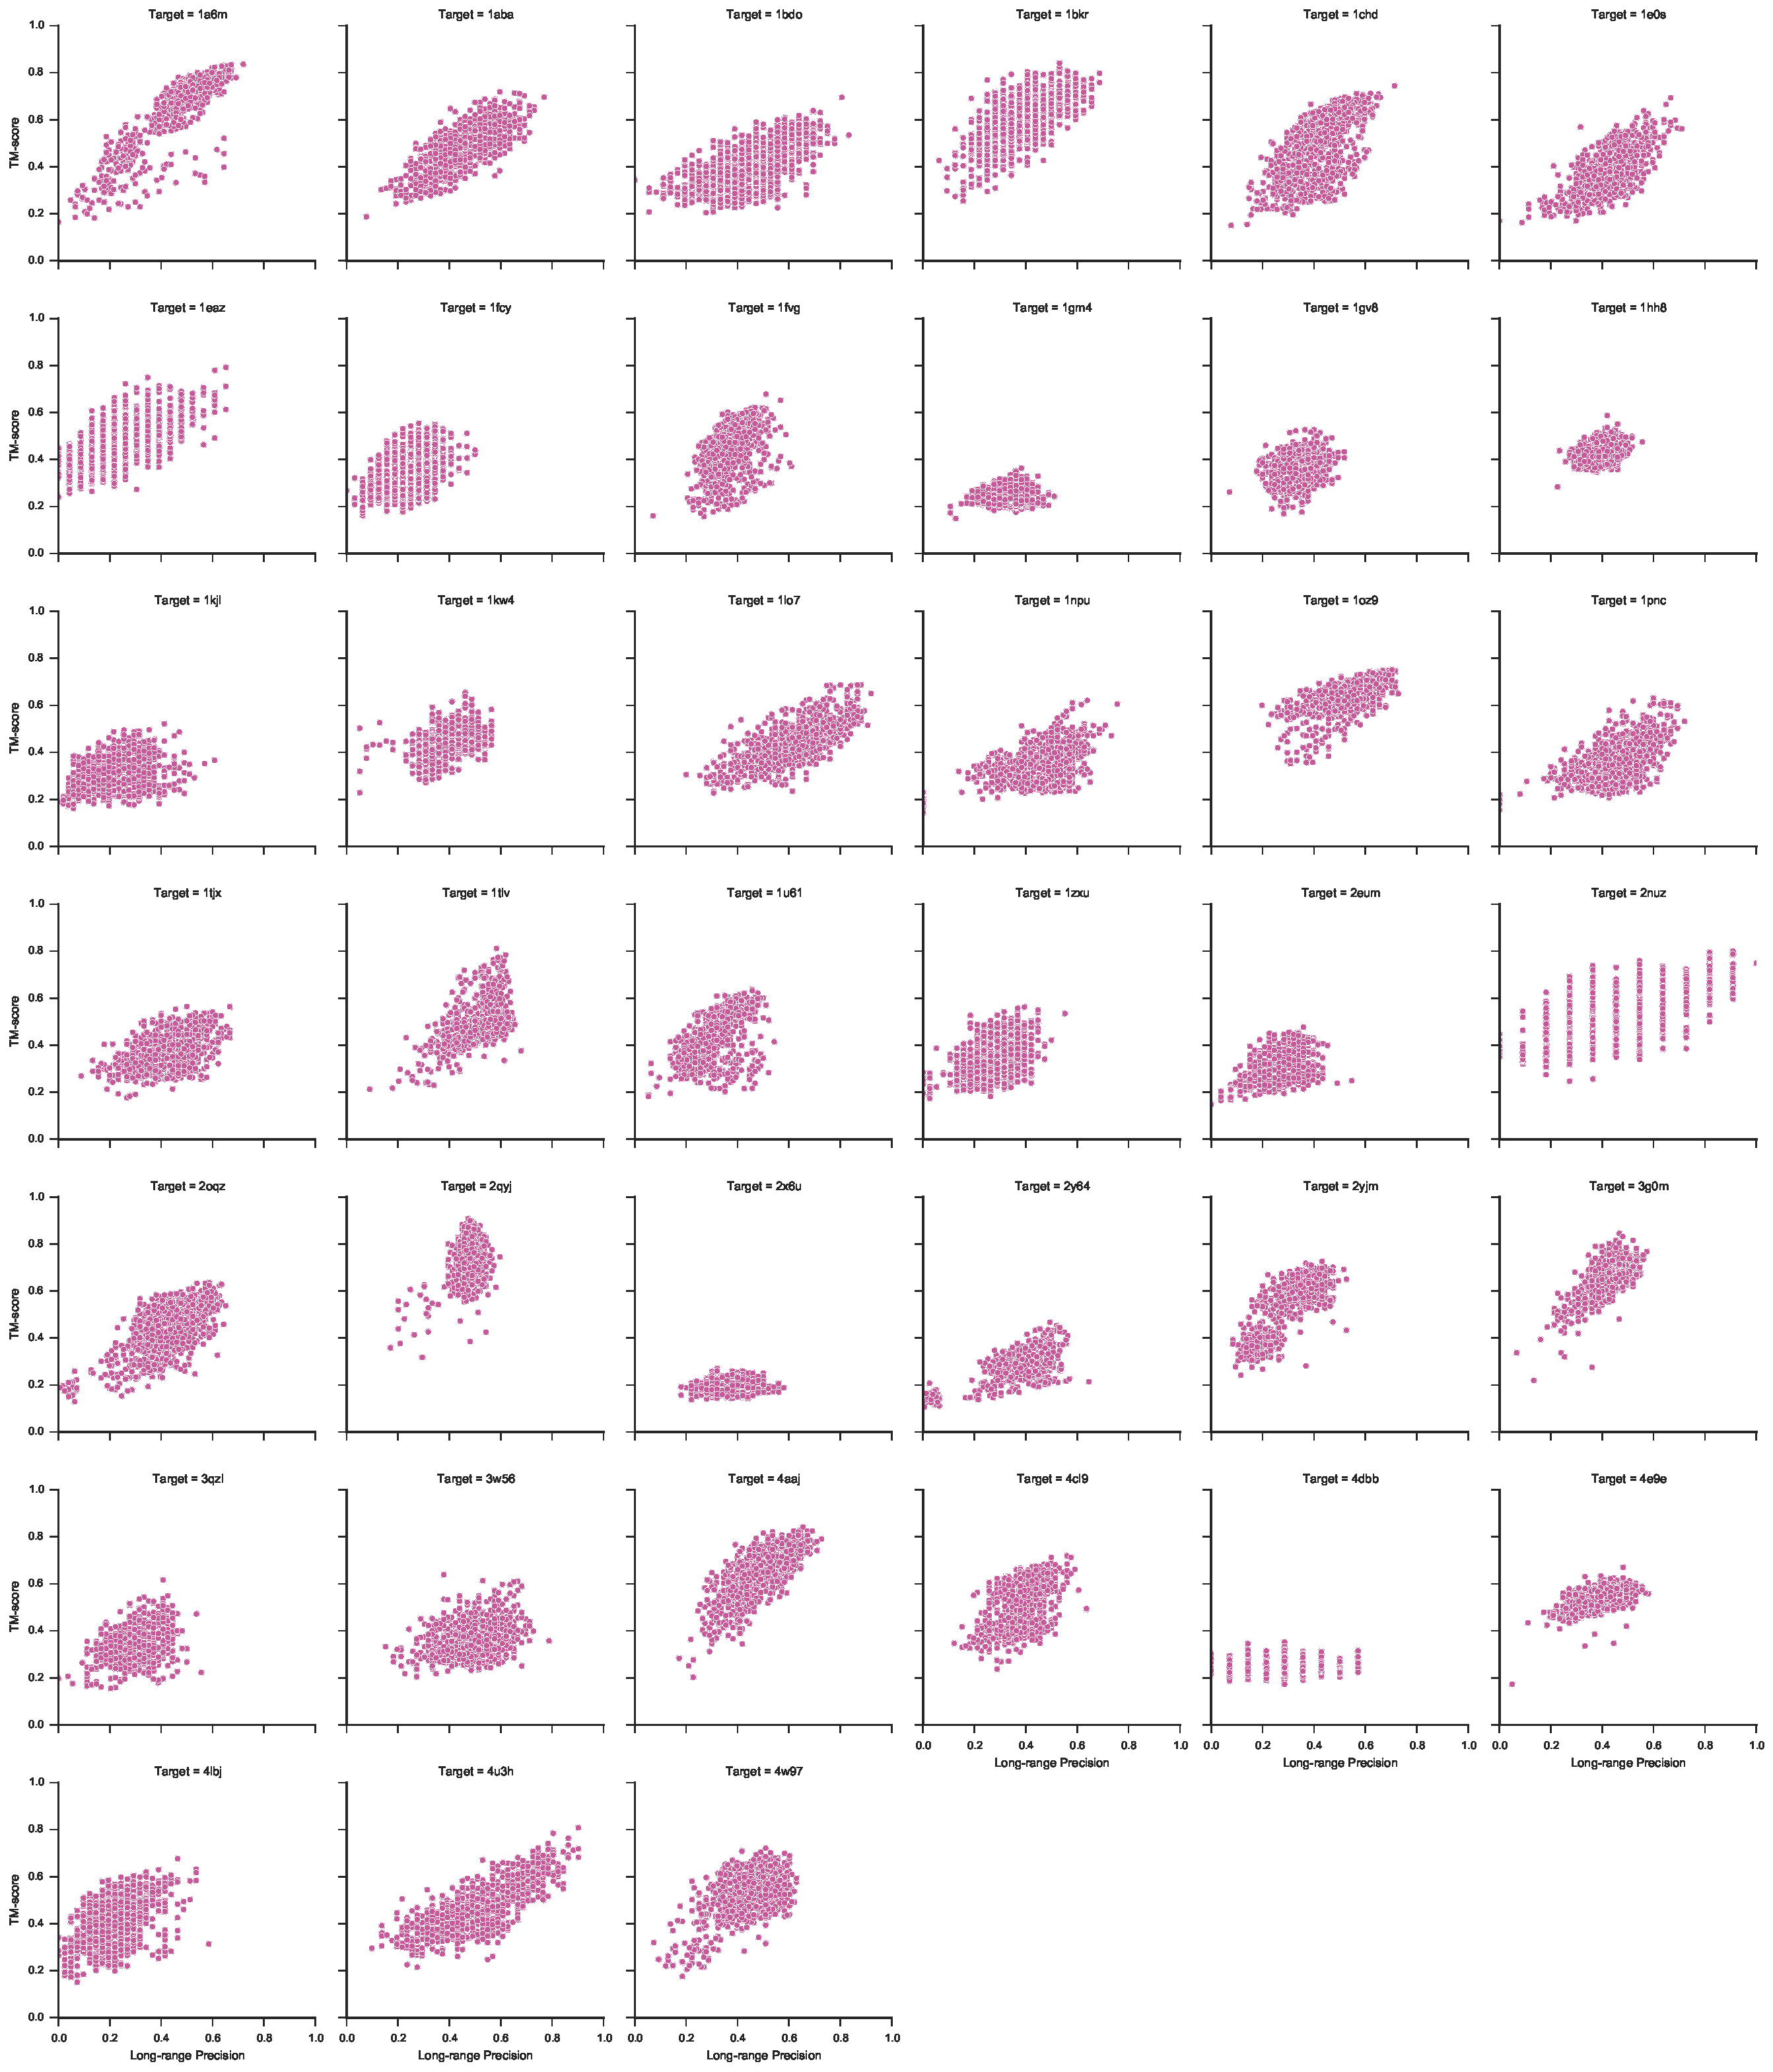
\includegraphics[width=\textwidth]{ample_decoys_pconsc2_lrprectm.pdf}
%         \caption{}
%         \label{fig:ample_decoys_pconsc2_lrprectm}
%     \end{subfigure}
%     \caption{Long-range contact precision and TM-score comparison for decoys generated with (a) CCMPRED, (b)
%     MEMBRAIN, (c) METAPSICOV, and (d) PCONSC2 contact predictions.}
%     \label{fig:ample_decoys_lrprectm}
% \end{figure}


% \subsection{Different subselection modes yield different final decoy sets}
%
% \section{Discussion}
